%%%%%%%%%%%%%%%%%%%%%%%%%%%%%%%%%%%%%%%%%%%%%%%%%%%%%%%%%%%%%%%%%%%%%%%%%%%%%%
%
% タイトル TeX用テンプレート 
% バージョン 2014-11-8 (Sat) 初版
% 作成者 Kouhei Ito
% 作成場所 
% 用途 2段組レポートの作成等
%
%%%%%%%%%%%%%%%%%%%%%%%%%%%%%%%%%%%%%%%%%%%%%%%%%%%%%%%%%%%%%%%%%%%%%%%%%%%%%%%%
\documentclass[a4paper]{jarticle}
\usepackage{sice-si}
\usepackage{amsmath} 
\usepackage[dvipdfmx]{graphicx}



%%%%%%%%%%%%%%%%%%%%%%%%%%%%%%%%%%%%%%%%%%%%%%%%%%%%%%%%%%%%%%%%%%%%%%%%%%%%%%%%

%%%%%%%%%%%%%%%%%%%%%%%%%%%%%%%%%%%%%%%%%%%%%%%%%%%%%%%%%%%%%%%%%%%%%%%%%%%%%%%%


\begin{document}

\title{超低重心6輪独立懸架ローバーの画像情報による自律走行}
\name{佐々井 翔也, 畠中 和久,  戸澗 健, 剱崎 健太郎, \\北山 天斗, 澤田 茂人, 伊藤 恒平 (金沢工業高等専門学校)}
\etitle{Ultra-low center of gravity six -wheel rover with Autonomous travel from the image information}
\ename{Shoya SASAI, Kazuhisa HATAKENAKA, Takeru TOMA Kentaro KENZAKI, \\Takato KITAYAMA , Shigeto SAWADA and Kouhei ITO}

\abst{本年度のつくばチャレンジでは、新たに開発中の台車の実環境での走行試験と画像により自律走行するための技術的知見を得ることを目標として参加した。これまでの台車が大型で重心も高く不安定であったため、輸送時に輸送コストを低く抑えられ、低重心で少しくらいの悪路でも走行可能な6輪独立懸架で6輪駆動の台車を作成した。また、自己位置推定と自律走行においては測域センサを活用してきたが、即行きセンサの役割を単眼カメラ画像に担わせることはできないかの検討を始めた。
}

\maketitle


%%%%%%%%%%%%%%%%%%%%%%%%%%%%%%%%%%%%%%%%%%%%%%%%%%%%%%%%%%%%%%%%%%%%%%%%%%%%%%%%
\section{はじめに}
%茨城県南部に位置するつくば市では毎年行われる「つくばチャレンジ」というロボットの大会がある.これはつくば市内の遊歩道等の実際の環境を移動ロボットに自律走行させる大会で,地域と研究者,教育者,学生が協力して行う,人間とロボットが共存する社会のための架け橋となる大会である. 
%自律走行には安定した走りと外の情報を得るための制御が必要である.
%前回のつくばチャレンジのロボットは重心が高いからこけた

前年度つくばチャレンジ2015ではロボットの重心が高かったため,凸凹道やコンクリートなどでロボットに傾きが発生しそのまま転倒しかける様子が見られた.
そこで,今回は地域住民に怪我や事故が発生しないようなロボットの走行方法と低重心の安定性に注目し,”超低重心6輪独立懸架ローバー”を制作する.また,自律走行を実現するために自身の位置を認識する手段が必要である.その手段としてカメラを用いることにした.カメラである利点として,安価なデバイスで周りの状況がわかる点などが挙げられる.特に、周りの状況がわかることで障害物を回避し,その場でマッピングし,自律走行をすることを目指した.

\section{ハードウェアの構成}
ハードウェアの構成をTable.\ref{tab:op}に示す.
\begin{table}[htp]
  \begin{center}
    \caption{ハードウェアの構成}
  \begin{tabular}{|c|c|} \hline
    構成要素 & メーカ・型番・スペックなど \\ \hline
    Mian PC & NVIDIA JETSON TK1 \\ \hline
    OS & Ubuntu 14.04 LTS \\ \hline
    camera & Panasonic HX-A1H \\ \hline
    Buttery & KyPOM KT5100 4S 35C \\ \hline
    Motor & MABUCHI MOTOR RS-555VC-5524 \\ \hline
    Motion Sensor & 東京航空計器株式会社 CSM-MG100\\ \hline

  \end{tabular}
    \label{tab:op}
  \end{center}
\end{table}


\section{超低重心6輪独立懸架ローバー}
\subsection{台車開発の狙い}
サスペンションを内蔵する台車を制作する.つくばチャレンジ2016では安全のための低重心を目標としているため,台車の全高を小さく設計することでその目標に尽くす.また今回のロボットの超低重心を実現するための数値をTable.\ref{tab:joken} に示す
%振動をできるだけ減らす,もしくはいなすような足回りの構造を開発する.
%そこで全体のズレを少なくするために6輪のそれぞれサスペンションの設置をし,それが大きくかさ張らないようにすることが必要である.
\begin{table}[htp]
  \begin{center}
    \caption{目標数値}
  \begin{tabular}{|c|c|c|c|} \hline
横幅 & 600mm以内  \\  \hline
長さ & 1000mm以内\\ \hline
高さ & 150mm以内 \\ \hline
    乗り越える段差 & およそ30mm  \\ \hline
  \end{tabular}
    \label{tab:joken}
  \end{center}
\end{table}

\subsection{サスペンションの概要}
製作するロボットはある程度の段差を超えるための上下できる機構が必要である.よって近年最も身近な上下機構を持つ機械として,車に利用されるサスペンションを参考にした.Fig.\ref{fig:doublewish}に示すダブルウィッシュボーン式サスペンションは上下のアームとショックアブソーバ,ばねからなるもので,レーシングカーに多く使用されている.Fig.\ref{fig:strat}に示すストラット式サスペンションと呼ばれるものはショックアブソーバとサスペンションを一体化したものをアッパーアームにしたもので,近年の車やミニ四駆などに使用されている.両方とも独立懸架で安定性や利便性に置いてはストラット式が大きく優るが,今回はコンパクトに構成することも必要なため,もともと上下アームで囲われているスペースを活かせることができそうなダブルウィッシュボーン式サスペンションを基礎として開発する.

\begin{figure}[htp]
 \begin{center}
  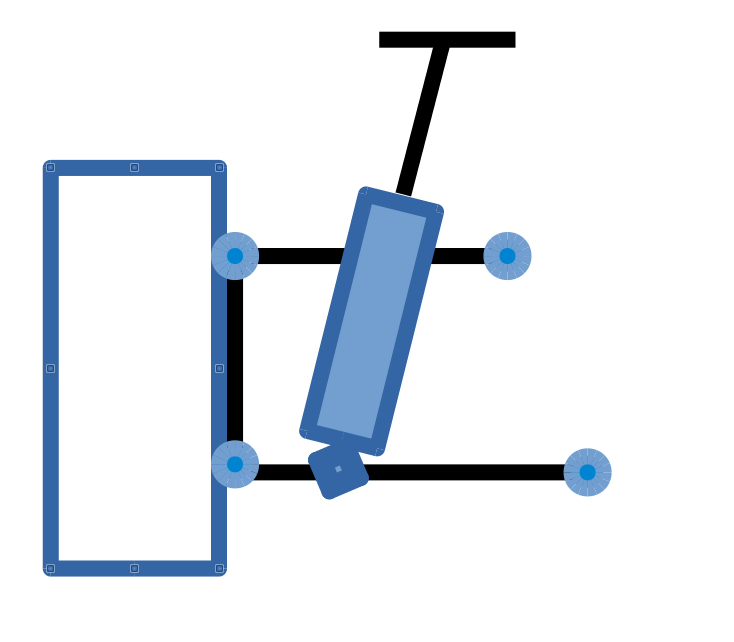
\includegraphics[width=50mm]{img/fig1.png}
  \caption{ダブルウィッシュボーン式サスペンション}
  \label{fig:doublewish}%ここに文章中で使用する名前を指定する
 \end{center}
\end{figure}

\begin{figure}[htp]
 \begin{center}
  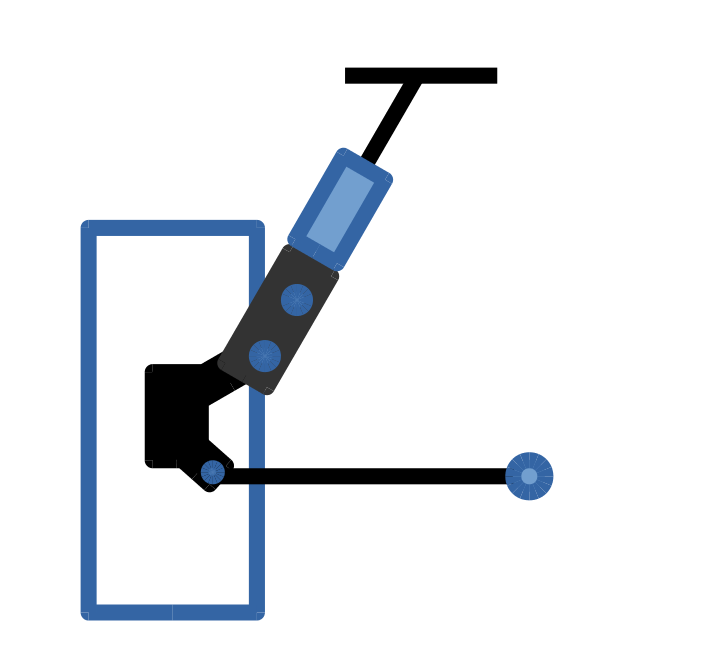
\includegraphics[width=40mm]{img/fig2.png}
  \caption{ストラット式サスペンション}
  \label{fig:strat}%ここに文章中で使用する名前を指定する
 \end{center}
\end{figure}

\subsection{台車の概要}

製作する”超低重心6輪独立懸架ローバー”(以下6輪ローバ)はFig.\ref{fig:rokurin}に示すとおり低重心であるがゆえにロボットそのものが平たく大きい物になる.そのままではメンテナンス性にかける他,運搬時に非常に不便なため,モータを持つドライブモジュール(以下Dモジュール)と指示塔であるコントロールモジュール(以下Cモジュール)に分解できるように台車を設計し,分解から組み立てを容易とするようにした.つまり2つのDモジュールと1つのCモジュールからなる1つの台車である.

\begin{figure}[htp]
 \begin{center}
  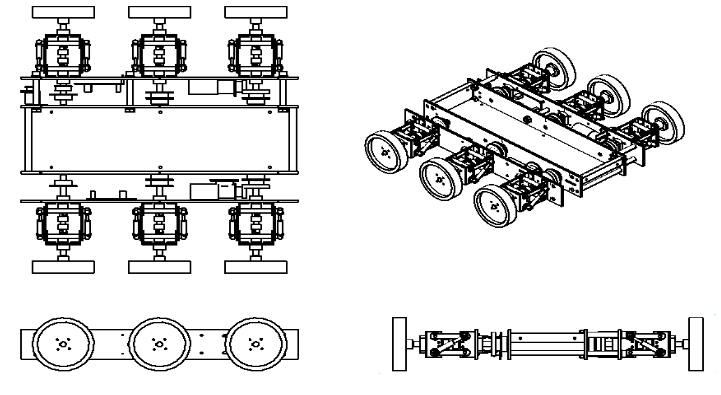
\includegraphics[height=51mm,width=80mm]{img/fig3.png}
  \caption{6輪ローバ}
  \label{fig:rokurin}%ここに文章中で使用する名前を指定する
 \end{center}
\end{figure}
%\subsection{設計}超低重心六輪独立懸架ローバ
%本項目ではサスペンションについて詳しく記す.

\subsection{サスペンションの配置}
%ダブルウィッシュボーン式サスペンションは便利ではあるが問題点も目立つ.例えばばねのストロークが少ない,ストロークを大きくしようとすれば車体との接続が困難になる,決められた場所にしか設置できない等,どれもスペースが大きく関係してくる.

台車の全高は小さくなるため,サスペンションの配置は小スペースに収めることが必要になる.そこでFig.\ref{fig:box}のように軸棒,ユニバーサルジョイント,車輪を上下のリンクと板を用いて1つの平行リンクをつくり,その平行リンクの両斜辺に2つ直接斜めに振動吸収となるばねを設置すれば車輪の径に左右されるものの従来のものよりスペースが小さく上下機構が得られるのではないかと考えた.

\begin{figure}[htbt]
 \begin{center}
  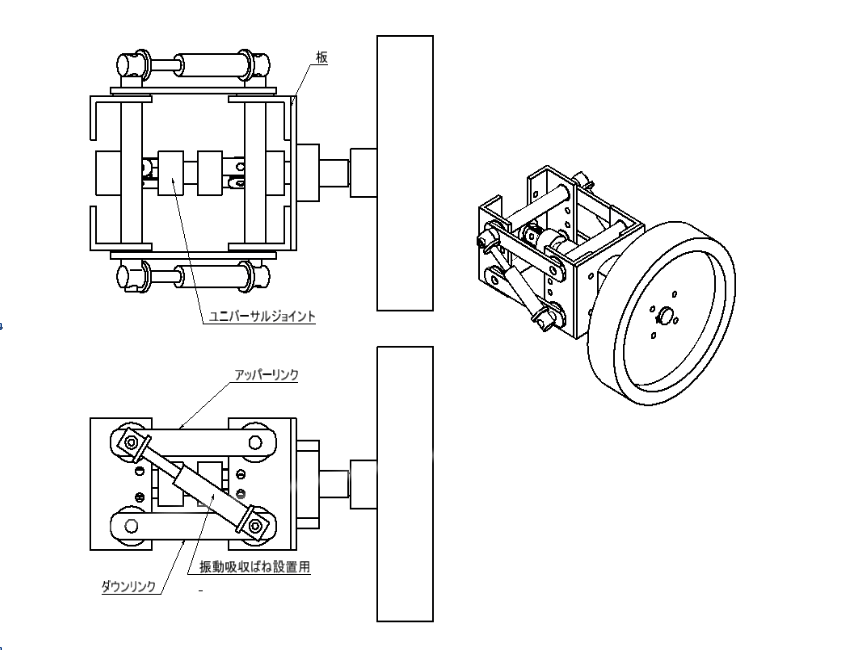
\includegraphics[width=60mm]{img/fig4.png}
  \caption{平行リンク}
  \label{fig:box}%ここに文章中で使用する名前を指定する
 \end{center}
\end{figure}

\subsection{ばねのストロークの算出}
Fig.\ref{fig:bix}に平行リンクの簡易Figを示す.また平行リンクが移動した際のFigをFig.\ref{fig:rink}示す.これらの数値よりサスペンションのストロークの長さを求める.サスペンションの全体長さは斜辺に設置するため余弦定理より
\begin{eqnarray}
   AC = b^2 & = & a_1^2+c^2-2a_1\cdot c\cdot cos\angle B \\
  b & = & \sqrt{38^2+60^2-2\cdot 38\cdot 60\cdot cos90} \\
    & = &71.022 ≒ 71.0[mm]
\end{eqnarray}
となる.また今回は30[mm]程度の障害物を乗り越える想定しているため,この平行リンクが点A,Bを回転軸として点C,Dが30[mm]上昇した際の平行四辺形の斜辺AC'を求める必要がある.平行リンクが移動してできるΔAC'Eの斜辺AC'はΔAD'Eの辺d'に等しい.よってAC'の式は余弦定理と代入法より
\begin{eqnarray}
	AE& = &d' =  \sqrt{a_2^2+e_1^2-2a_2\cdot e\cdot cos\angle D} \\
	d' & = & c' \\
	AC'&= &e_2  =  \sqrt{c'^2+a_3^2-2\cdot c'\cdot a_3\cdot cos\angle E}
\end{eqnarray}
となる.またΔAD'Eの\angle Aは30[mm]上がった際に30[deg]になることから,斜辺AC'は
\begin{eqnarray}
	d' &=& \sqrt{30^2+60^2-2\cdot 30\cdot 60\cdot cos\angle 60} \\
	d'&=&30\sqrt{3}=c' \\
	AC'&= &e_2  =  \sqrt{c'^2+a_3^2-2\cdot c'\cdot a_3\cdot cos\angle E}  \\
	AC' &=& \sqrt{(30\sqrt{3})^2+8^2-2\cdot 30\sqrt{3}\cdot 8\cdot cos90} \\
	& = & 52.574 ≒ 52.6 [mm]
\end{eqnarray}
となる. \\
サスペンションは伸縮するものであり,それはこれらの辺ACと辺AC'の差分だけ変化することになる.今回の値から変化値x≒18[mm]程度の変化があることが確認された.以上のAC,AC',xを用いてサスペンションの細かい設計を行う.

\begin{figure}[htp]
 \begin{center}
  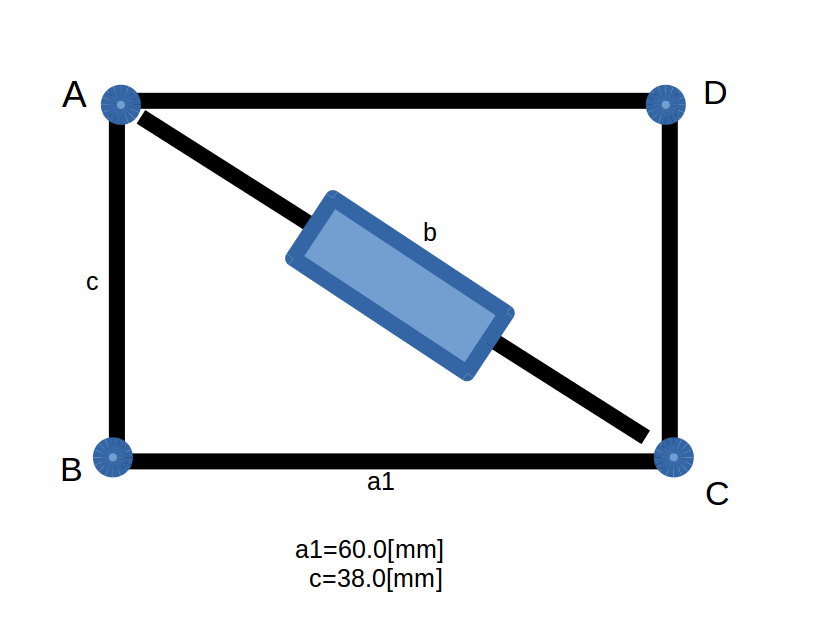
\includegraphics[width=60mm]{img/fig5.png}
  \caption{平行リンク簡易図}
  \label{fig:bix}%ここに文章中で使用する名前を指定する
 \end{center}
\end{figure}


\begin{figure}[htp]
 \begin{center}
  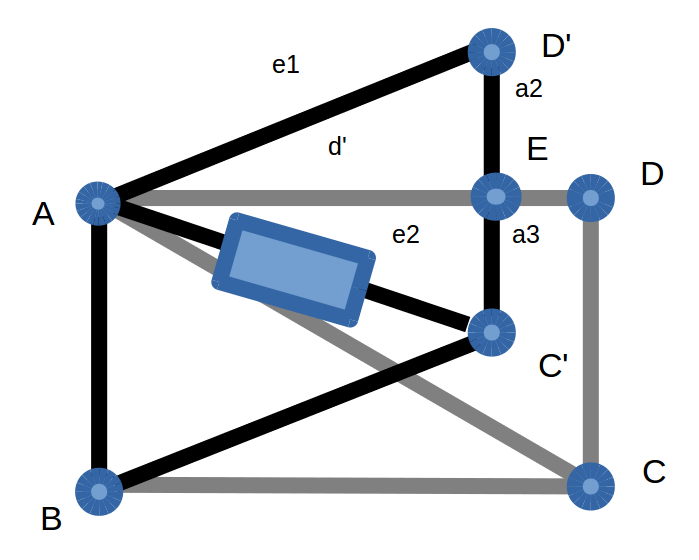
\includegraphics[width=60mm]{img/fig6.png}
  \caption{平行リンクの移動量変化}
  \label{fig:rink}%ここに文章中で使用する名前を指定する
 \end{center}
\end{figure}

\subsection{ばね定数の算出}
サスペンションには路面の凹凸を車体に伝えない緩衝装置としての機能としてばねが必要であるため,フックの法則よりばねを選定する. \\
平行リンクの点A,Bをそれぞれ固定支点と考えて計算を行う.Fig.\ref{fig:fbd}に Free Body Diagram(FBD)を示す.Fig.\ref{fig:fbd}よりスラスト方向荷重x,ラジアル方向荷重y,モーメントMの式はそれぞれ

\begin{eqnarray}
	x & = & R_AX+R_BX=0 \\
	y & = & R_AY+R_BY+F=0 \\
	M & = & BC\cdot F-AB\cdot R_AX=0
\end{eqnarray}
となる.更に点A,B,Cそれぞれの力は以下のようになる.

\subsubsection{点Aでの力学計算}
点AではFig.\ref{fig:bai}より以下のように計算できる.
\begin{eqnarray}
	R_AX+FAC\cdot cosθ & = & 0 \\
	R_AY & = & FAC\cdot sinθ 
\end{eqnarray}
\subsubsection{点Bでの力学計算}
点BはFig.\ref{fig:bai}より以下のように計算できる.
\begin{eqnarray}
	R_BX+FBC & = & 0 \\
	R_BY & = & 0
\end{eqnarray}
\subsubsection{点Cでの力学計算}
点CはFig.\ref{fig:bai}より以下のように計算できる.
\begin{eqnarray}
	FAC\cdot cosθ+FBC & = & 0 \\
	F+FAC\cdot sinθ & = & 0
\end{eqnarray}
\subsubsection{力学計算まとめ}
上記で求めた式より,ACにかかる力FACの式を計算する.
FACは式(14)と式(18)より
\begin{eqnarray}
	R_AY+F & = & 0 \\
		F & = & -R_AY 
\end{eqnarray}
\begin{eqnarray}
	    R_AY & = & FAC\cdot sinθ \\
		FAC & = & \frac{F}{sinθ} [N] 
\end{eqnarray}
\begin{eqnarray}
	F+FAD\cdot sinθ & = & 0 \\
	FAC & = & \frac{F}{sinθ} [N]
\end{eqnarray}

となることが確認できる. \\
力FAC[N]はばね全体に掛る力なので,これをばね1個辺りに加わる力に除算する必要がある.今回作成する6輪ローバは1輪に2つのばねを持つため,ばねを合計で12個保有する.よってばね1個にかかる力FAC[N]は

\begin{eqnarray}
	FAC & = & \frac{F}{sinθ}\cdot \frac{1}{12} [N]
\end{eqnarray}

となる.今回は重量が15kgになると想定して,ばね定数を求めると
\begin{eqnarray}
	FAC & = & \frac{F}{sinθ}\cdot \frac{1}{12} \\
	FAC & = & \frac{15 \cdot  9.81}{sin30}\cdot \frac{1}{12} [N] \\
	     & =& 24.525[N] 
\end{eqnarray}
	{これより} 
\begin{eqnarray}
	k& = &  \frac{F}{x} \\
	k& = &  \frac{24.525}{18} \\
	 & = & 1.3625 [N/mm]
\end{eqnarray}
となる.よってばね定数は1.0[N/mm]の物を採用する.

\begin{figure}[htp]
 \begin{center}
  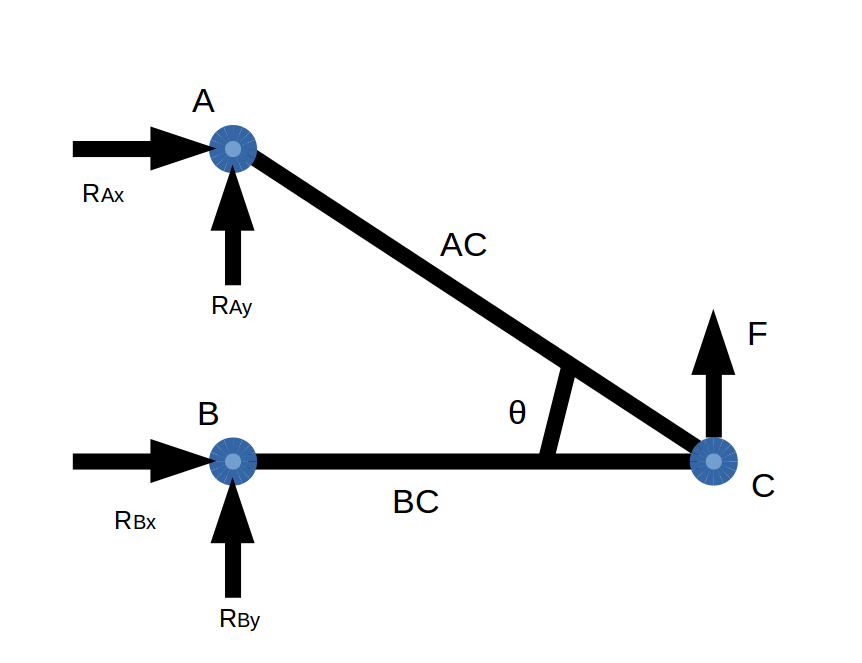
\includegraphics[width=50mm]{img/fig7.png}
  \caption{FBD}
  \label{fig:fbd}%ここに文章中で使用する名前を指定する
 \end{center}
\end{figure}

\begin{figure}[htp]
 \begin{center}
  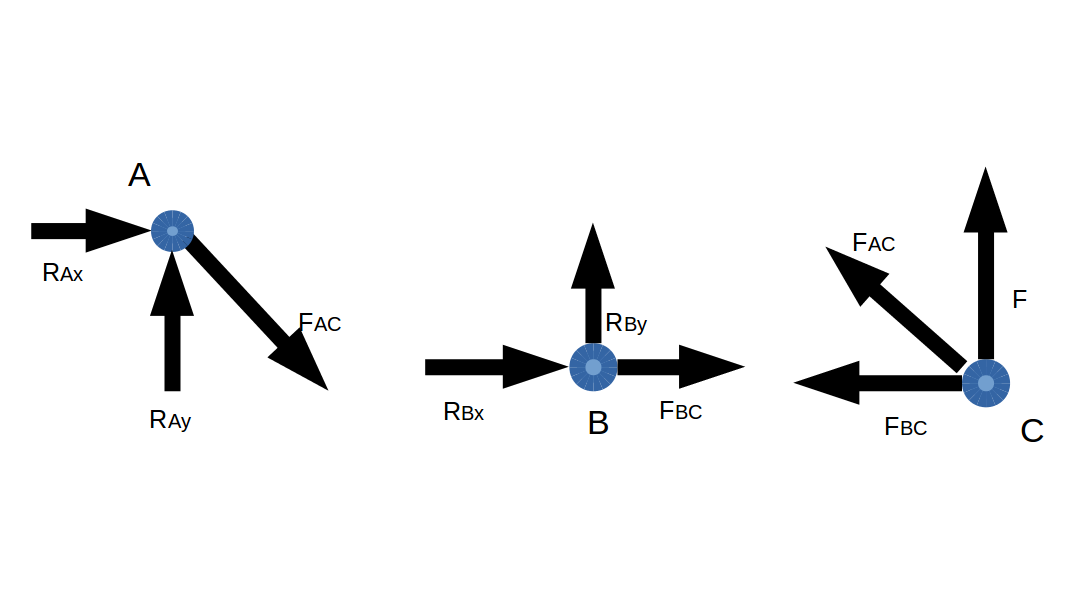
\includegraphics[width=70mm]{img/fig8.png}
  \caption{各点にかかる力}
  \label{fig:bai}%ここに文章中で使用する名前を指定する
 \end{center}
\end{figure}

%\subsection{サスペンションの材質}
%サスペンションの大まかな大きさが判明したので細かい設計を行う.設計図をfig\ref{fig:saspention}に示す.サスペンションは加工の行いやすさと軽さを踏まえてアルミニウム(Al)を用いて作成する.
%\begin{figure}[htp]
 %\begin{center}
  %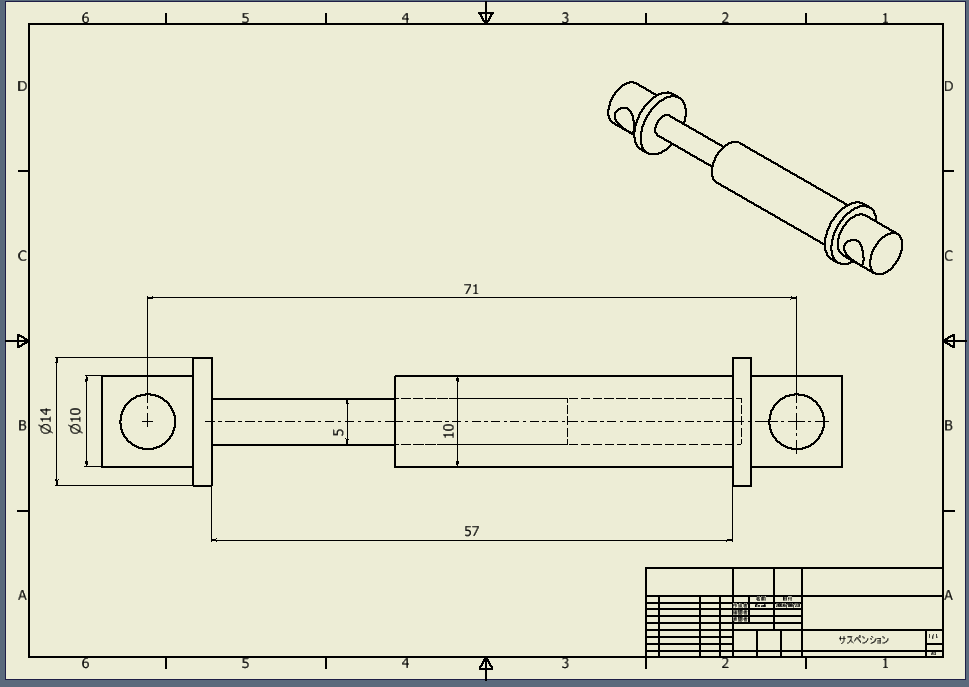
\includegraphics[width=60mm]{img/fig9.png}
  %\caption{サスペンションの設計図}
  %\label{fig:saspention}%ここに文章中で使用する名前を指定する
 %\end{center}
%\end{figure}

\subsection{走行実験結果}
今回作成したサスペンションを用いて台車を試走させたところばねによる衝撃緩和が確認された.しかし,速度の上昇加減によってばねによる振動が発生したのが確認された.


\section{カメラ画像からの環境認識}
\subsection{3次元復元}
3次元復元とは,画像上の2次元座標から3次元座標を得ることである.これは、カメラの焦点距離と画像のセンター座標を含む内部パラメータ行列を使用して行う.また,Mをカメラの内部パラメータ行列,[R|t]を並進・回転の同次変換行列としその関係式を下記に示す.
\begin{equation}
\left(
    \begin{array}{c}
      u \\
      v \\
      1 
    \end{array}
  \right)=M[R|t]\left(
    \begin{array}{c}
      X \\
      Y \\
      Z \\
      W
    \end{array}
  \right)
\end{equation}
実際の3次元座標はXYZをそれぞれWで割ることにより求まる.

3次元復元の流れを下記に示す.

\subsection{カメラの校正}
\subsubsection{カメラの校正}
カメラの校正とはレンズによって生じる歪みやレンズの焦点距離などのパラメータを推定するものであり,OpenCVの校正アルゴリズムではピンホールカメラモデルを想定している.

\subsubsection{ピンホールカメラモデル}
ピンホールカメラとはピンホール(光学中心)を開けた箱の内側に外界の風景を上下左右反転して映ることを利用した初期のカメラである.そして,ピンホールを通る光線だけで投影面への結像をモデル化したのがピンホールカメラモデルであり,そのモデルを図1に示す.

\begin{figure}[htbp]
 \begin{center}
  \includegraphics[width=60mm]{image/pinhole.png}
  \caption{ピンホールカメラモデル}%図題
  \label{fig:02}%文章中の名前
 \end{center}
\end{figure}

fig\ref{fig:02}よりピンホールを通過した光線は画像面の1点と交わり,そこで像を結ぶ.この像は元の画像を逆転させたものになるため画像面を光学中心より前に移すと良い.また画像面を移すことを透視投影と呼ぶ.

\subsubsection{透視変換}
カメラの結像に関する座標系をFig.\ref{fig:03},カメラと画像の座標系をFig.\ref{fig:04}に示す.

\begin{figure}[htbp]
 \begin{center}
  \includegraphics[width=60mm]{image/camera1.png}
  \caption{カメラの結像に関する座標系}%図題
  \label{fig:03}%文章中の名前
 \end{center}
\end{figure}

\begin{figure}[htbp]
 \begin{center}
  \includegraphics[width=60mm]{image/camera2.png}
  \caption{カメラと画像の座標系}%図題
  \label{fig:04}%文章中の名前
 \end{center}
\end{figure}

光学中心Ocから画像面までの距離(焦点距離)をfとすると,
この座標系で(x,y,z)にある空間の点に対応する像は相似の関係(fx/z,fy/z,f)となる.
画像面上の点(fx/z,fy/z)の透視変換は

\begin{equation}
\left(
    \begin{array}{c}
      x \\
      y \\
      z 
    \end{array}
  \right)=\frac{f}{z} \left(
    \begin{array}{c}
      x \\
      y \\
       
    \end{array}
  \right)
\end{equation}
となる.つまり,カメラに対する相対的な位置によって,結像される位置が決まる.

\subsection{Essential Matrixを求める}
Essential Matrix(E)とは2つのカメラを実空間で関連付ける,平行移動と回転に関する情報を含む行列である.また,Essential Matrixを下記に示す.

\begin{equation}
       E = \left(
    \begin{array}{cccc}
      r _{11} & r _{12} & r _{13} & t_1\\
      r _{21} & r _{22} & r _{23} & t_2\\
      r _{31} & r _{32} & r _{33} & t_3\\

    \end{array}
  \right)
\end{equation}
OpenCVでEssential Matrixを求める際に利用されている手法は8点法{\scriptsize[1]}もしくはその改良版の5点法である.
カメラのパラメータが既知の場合,5点法を用いることでEssentiinal Matrixを求めることができる.


\subsection{回転行列・並進行列を求める}
回転行列Rは3×3,並進行列tは3×1の行列で表される.
式3よりEssential Matrixは回転行列Rと並進行列tを1つにまとめた4×4の行列[R|t]で構成されていることが分かる.よってEssential Matrixを分解することにより,回転行列Rと並進行列tを求めることができる.

\subsection{三角測量}
対応付けされた2点間の座標と並進,回転を求めることでFig.\ref{fig:05}のように二次元座標を三次元復元することができる.

\begin{figure}[htbp]
 \begin{center}
  \includegraphics[width=60mm]{image/index.jpeg}
  \caption{三角測量}%図題
  \label{fig:05}%文章中の名前
 \end{center}
\end{figure}

左画像の中心Q{\scriptsize L},右画像の中心Q{\scriptsize R},特徴点Pをつなげることで三角形を作ると,特徴点Pの座標は
式(\ref{eq:1}), 式(\ref{eq:2}), 式(\ref{eq:3})のような関係が成り立つ.

\begin{equation}
 x=\frac {R・d・x_{L}}{X_{L}-X_{R}}
 \label{eq:1}
\end{equation}

\begin{equation}
 y=\frac {R・d・y_{L}}{X_{L}-X_{R}}
 \label{eq:2}
\end{equation}

\begin{equation}
 z=\frac {R・d・f}{X_{L}-X_{R}}
 \label{eq:3}
\end{equation}


式(\ref{eq:1}), 式(\ref{eq:2}), 式(\ref{eq:3})より,特徴点Pの三次元座標を得ることができる.


\section{考察}
サスペンションが正常に機能するならば,つくば市街の道路を安定的に走行することが期待できる.更に今回の走行速度は1km/h(0.28m/s)という低速なため,ばねのみでもさほどの問題は感じられないと考える.また,カメラで3次元復元を行い得られた座標情報は,対応付けられた点情報とカメラの内部パラメータが正確であれば正しいといえる.さらに,座標情報が正確であれば地図データや現在の位置も正確に求まる.また,カメラの内部パラメータは校正により求まる.よって,対応付けられた点情報の正確性を高めることが最も重要であると言える.


\section{おわりに}
今回作成したダブルウィッシュボーン式サスペンションを基にしたサスペンションは小さい範囲に機能を積むことで本体の低位置を確立し,走行する上での障害物に対する振動を小さく抑えることができた.しかし今回はスペースと加工工程の都合上ショックアブソーバの取り付けができなかったため,高速度での使用になるとばねが伸縮し続け,本体が弾むことが予想される.その問題を解消するため,ショックアブソーバの取り付けがこれからの課題となる.また,カメラによる3次元復元では地図を作成することに成功した.地図データと3次元復元で得た自己位置のデータを比較し,より正確な位置情報を得ることが今後の課題である.

\section*{参考文献}
[1]Bradski,Kaehler:詳解 OpenCV,433,株式会社オライリー・ジャパン(2012)


\end{document}

